\documentclass[a4paper,11pt]{article}

% Package imports - reordered and fixed for local compilation
\usepackage[T1]{fontenc}
\usepackage[utf8]{inputenc}
\usepackage{latexsym}
\usepackage{xcolor}
\usepackage{float}
\usepackage{ragged2e}
\usepackage[empty]{fullpage}
\usepackage{wrapfig}
\usepackage{tabularx}
\usepackage{titlesec}
\usepackage{geometry}
\usepackage{marvosym}
\usepackage{verbatim}
\usepackage{enumitem}
\usepackage{fancyhdr}
\usepackage{multicol}
\usepackage{graphicx}
\usepackage{microtype}
\usepackage{array} % Required for vertical centering in tables

% Font packages - using more compatible options
\usepackage{lmodern} % Latin Modern fonts (replacement for cfr-lm)
\usepackage{fontawesome} % FontAwesome icons (more compatible than fontawesome5)

% Hyperref should be loaded last
\usepackage[hidelinks]{hyperref}

% tcolorbox - using basic version for better compatibility
\usepackage{tcolorbox}

% Color definitions
\definecolor{darkblue}{RGB}{0,0,139}

% Page layout
\geometry{left=1.4cm, top=0.8cm, right=1.2cm, bottom=1cm}
\setlength{\multicolsep}{0pt} 
\pagestyle{fancy}
\fancyhf{} % clear all header and footer fields
\fancyfoot{}
\renewcommand{\headrulewidth}{0pt}
\renewcommand{\footrulewidth}{0pt}
\setlength{\footskip}{4.08pt}

% Hyperlink setup
\hypersetup{
    colorlinks=true,
    linkcolor=darkblue,
    filecolor=darkblue,
    urlcolor=darkblue,
}

% Custom box settings - simplified for better compatibility
\tcbset{
    frame code={},
    center title,
    left=0pt,
    right=0pt,
    top=0pt,
    bottom=0pt,
    colback=gray!20,
    colframe=white,
    width=\dimexpr\textwidth\relax,
    enlarge left by=-2mm,
    boxsep=4pt,
    arc=0pt,outer arc=0pt,
}

% URL style
\urlstyle{same}

% Text alignment
\raggedright
\setlength{\tabcolsep}{0in}

% Section formatting
\titleformat{\section}{
  \vspace{-4pt}\scshape\raggedright\large\bfseries
}{}{0em}{}[\color{black}\titlerule \vspace{-7pt}]

% Custom commands
\newcommand{\resumeItem}[2]{
  \item{
    \textbf{#1}{\hspace{0.5mm}#2 \vspace{-0.5mm}}
  }
}

% New command for different font sizes and indentation in bullet points
\newcommand{\resumeItemMain}[1]{
  \item #1
}

\newcommand{\resumeItemSub}[1]{
  \item[] \hspace{0.05mm} $\diamond$ {\small #1}
}

\newcommand{\resumeItemSubSub}[1]{
  \item[] \hspace{0.1mm} $\ast$ {\footnotesize #1}
}

\newcommand{\resumePOR}[3]{
\vspace{0.5mm}\item
    \begin{tabular*}{0.97\textwidth}[t]{l@{\extracolsep{\fill}}r}
        \textbf{#1}\hspace{0.3mm}#2 & \textit{\small{#3}} 
    \end{tabular*}
    \vspace{-2mm}
}

% Modified resumeSubheading to move dates to right margin
\newcommand{\resumeSubheading}[4]{
\vspace{0.5mm}\item
    \begin{tabular*}{0.98\textwidth}[t]{l@{\extracolsep{\fill}}r}
        \textbf{#1} & \textit{\footnotesize{#4}} \\
        \textit{\footnotesize{#3}} & \footnotesize{#2} \\
    \end{tabular*}
    \vspace{-2.4mm}
}

\newcommand{\resumeProject}[4]{
\vspace{0.5mm}\item
    \begin{tabular*}{0.98\textwidth}[t]{l@{\extracolsep{\fill}}r}
        \textbf{#1} & \textit{\footnotesize{#3}} \\
        \footnotesize{\textit{#2}} & \footnotesize{#4}
    \end{tabular*}
    \vspace{-2.4mm}
}

\newcommand{\resumeSubItem}[2]{\resumeItem{#1}{#2}\vspace{-4pt}}

% Bullet point symbols for different levels
\renewcommand{\labelitemi}{\raisebox{0.2ex}{\large$\bullet$}}
\renewcommand{\labelitemii}{$\vcenter{\hbox{\scriptsize$\circ$}}$}
\renewcommand{\labelitemiii}{$\vcenter{\hbox{\tiny$\diamond$}}$}
\renewcommand{\labelitemiv}{$\vcenter{\hbox{\scriptsize$\ast$}}$}

% List environment commands - simplified to avoid nesting issues
\newcommand{\resumeSubHeadingListStart}{\begin{itemize}[leftmargin=*,labelsep=0.1mm]}
\newcommand{\resumeHeadingSkillStart}{\begin{itemize}[leftmargin=*,itemsep=1.7mm, rightmargin=2ex]}
\newcommand{\resumeItemListStart}{\begin{itemize}[leftmargin=*,labelsep=1mm,itemsep=0.5mm]}

\newcommand{\resumeSubHeadingListEnd}{\end{itemize}\vspace{2mm}}
\newcommand{\resumeHeadingSkillEnd}{\end{itemize}\vspace{-2mm}}
\newcommand{\resumeItemListEnd}{\end{itemize}\vspace{-2mm}}

\newcommand{\cvsection}[1]{%
\vspace{2mm}
\begin{tcolorbox}
    \textbf{\large #1}
\end{tcolorbox}
    \vspace{-4mm}
}

\newcolumntype{L}{>{\raggedright\arraybackslash}X}%
\newcolumntype{R}{>{\raggedleft\arraybackslash}X}%
\newcolumntype{C}{>{\centering\arraybackslash}X}%

% Commands for icon sizing and positioning - simplified
\newcommand{\socialicon}[1]{\raisebox{-0.05em}{\resizebox{!}{1em}{#1}}}
\newcommand{\ieeeicon}[1]{\raisebox{-0.3em}{\resizebox{!}{1.3em}{#1}}}

% Font options - using more compatible font commands
\newcommand{\headerfonti}{\sffamily} % Sans serif
\newcommand{\headerfontii}{\rmfamily} % Roman (serif)
\newcommand{\headerfontiii}{\ttfamily} % Typewriter

% Define personal information
\newcommand{\name}{Syahrul Fathoni Ahmad} % Your Name
\newcommand{\course}{Bachelor of Engineering} % Your Course
\newcommand{\roll}{XXXXXX} % Your Roll No.
\newcommand{\phone}{8999109204} % Your Phone Number
\newcommand{\emaila}{syahrulfa1106@gmail.com} % Email 1
\newcommand{\emailb}{officialemail@nitp.ac.in} % Email 2
\newcommand{\github}{still-breath} % Github
\newcommand{\website}{https://syahrul-fathoni.vercel.app} % Website
\newcommand{\linkedin}{syahrulahmad} % LinkedIn

\begin{document}
\sloppy
\rmfamily % Using standard roman family instead of cmr

%----------HEADING-----------------
\parbox{2.35cm}{%
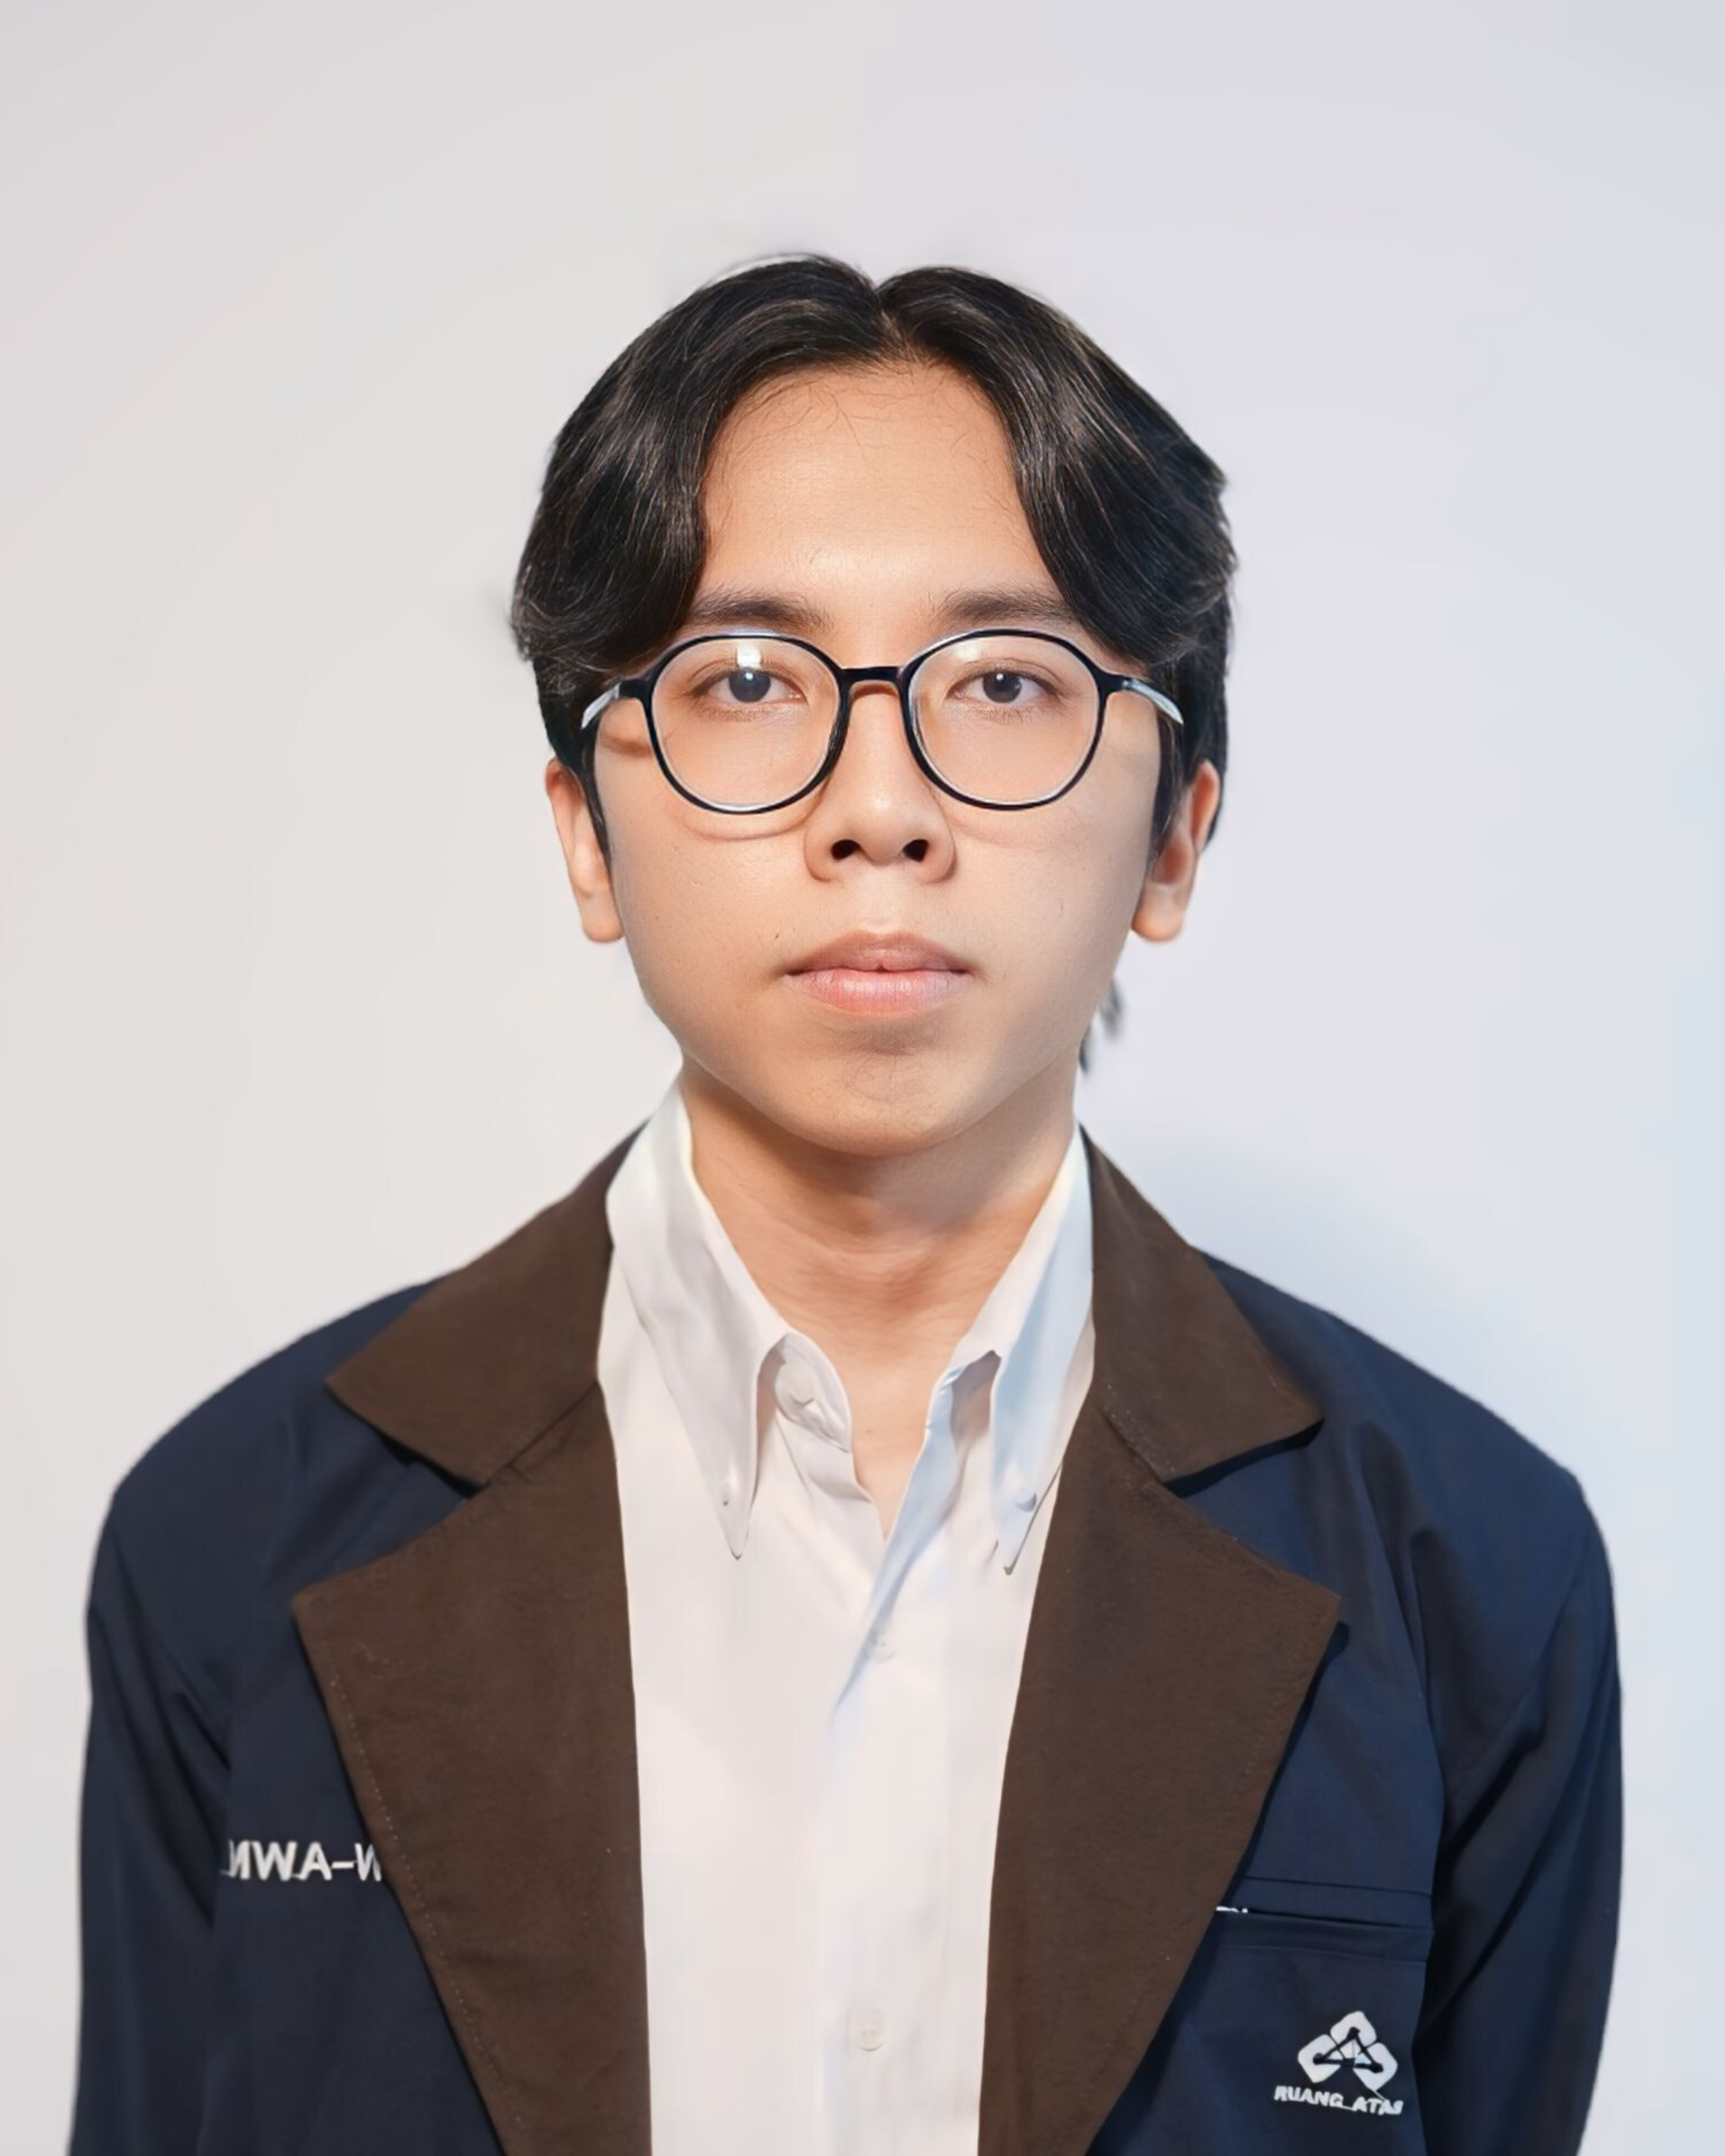
\includegraphics[width=2cm,clip]{91.png}
}
\parbox{\dimexpr\linewidth-2.8cm\relax}{
\begin{tabularx}{\linewidth}{L r}
  \textbf{\LARGE \name} & +62-\phone \\
  \course & \href{mailto:\emailb}{\emaila} \\
  Computer Engineering & \href{https://www.linkedin.com/in/\linkedin}{linkedin.com/in/\linkedin} \\
  Institut Teknologi Sepuluh Nopember, Surabaya
  & \href{https://github.com/\github}{github.com/\github} \\
  & \href{https://syahrul-fathoni.vercel.app}{syahrul-portfolio-web}
\end{tabularx}
}
\vspace{-2mm}

\section{\textbf{Education}}
\vspace{1mm}
\setlength{\tabcolsep}{5pt}
\begin{tabularx}{\textwidth}{|>{\centering\arraybackslash}X|>{\centering\arraybackslash}p{8cm}|>{\centering\arraybackslash}p{3cm}|>{\centering\arraybackslash}p{2.5cm}|}
  \hline
  \textbf{Degree} & \textbf{Institute} & \textbf{Current CGPA} & \textbf{Year} \\
  \hline
  S.T., Teknik Komputer & Institut Teknologi Sepuluh Nopember, Surabaya & 3.41/4.0 & Aug 2025 \\ 
  \hline
\end{tabularx}
\vspace{-4mm}

\section{\textbf{Skills}}
\vspace{-0.4mm}
\resumeHeadingSkillStart
    \resumeSubItem{Full-Stack Development}{: Python, Go (Golang), JavaScript, React.js, Node.js, Express.js, Flask, API, SQL, MongoDB, Three.js, HTML/CSS}
    \resumeSubItem{AI \& IoT Systems}{: PyTorch, TensorRT, YOLO, LSTM, NLP Jetson Nano, ESP32, Arduino, C++, PyQt, RTMP/RTSP Streaming}
    \resumeSubItem{DevOps \& Cloud}{: Git, Docker, VPS Hosting \& Configuration, Vercel, Azure, Nginx, Apache}
\resumeHeadingSkillEnd
\vspace{-2mm}

\section{\textbf{Work Experiences}}
\vspace{-0.4mm}
\resumeSubHeadingListStart
\resumeSubheading
    {Freelance}{Hybrid}
    {Freelancer}{2022 - Present}
    \resumeItemListStart

        \item
        \begin{tabular*}{\linewidth}{@{}l@{\extracolsep{\fill}}r@{}}
        \textbf{Retrux-Shelf-Eye (AI Inventory Management System):} & {\footnotesize\textit{Aug 2025 - Present}} \\
        {\footnotesize\textit{Tools:} Python, PyQt, PyTorch} & %{\footnotesize\href{https://github.com/still-breath/retrux-shelf-eye}{\textcolor{darkblue}{GitHub}}}
        \end{tabular*}
        \vspace{-0.8em}
        \resumeItemListStart
            \resumeItemSub{Developed a real-time shelf stock monitoring application using Python, with a user interface built in \textbf{PyQt}.}
            \resumeItemSub{Implemented an advanced object detection model (\textbf{RT-DETR}) using \textbf{SAHI} for sliced inference.}
            \resumeItemSub{Engineered key software utilities based on client needs, including \textbf{multi-camera support} and dynamic directory management.}
        \resumeItemListEnd
        \vspace{0.5em}

        \item
        \begin{tabular*}{\linewidth}{@{}l@{\extracolsep{\fill}}r@{}}
        \textbf{JAREE ITS (Academic Journal Platform):} & {\footnotesize\textit{July 2025 - Present}} \\
        {\footnotesize\textit{Tools:} OJS, PHP, MySQL, CSS} &% {\footnotesize\href{https://github.com/still-breath/container-optimizer}{\textcolor{darkblue}{GitHub}}}
        \end{tabular*}
        \vspace{-0.8em}
        \resumeItemListStart
            \resumeItemSub{Orchestrated a seamless, live migration of the OJS platform (v2 to v3), ensuring service continuity for \textbf{30k+ users} while upgrading a database of \textbf{597k+ records}.}
            \resumeItemSub{Engineered the complete academic peer-review workflow and developed a \textbf{custom front-end theme} to enhance user experience.}
        \resumeItemListEnd

        \item
        \begin{tabular*}{\linewidth}{@{}l@{\extracolsep{\fill}}r@{}}
        \textbf{Padel-Clipper (IoT Video Highlight System):} & {\footnotesize\textit{Aug 2025}} \\
        {\footnotesize\textit{Tools:} Python, Flask, ESP32, Express.js, PHP} & %{\footnotesize\href{https://github.com/still-breath/padel-clipper}{\textcolor{darkblue}{GitHub}}}
        \end{tabular*}
        \vspace{-0.8em}
        \resumeItemListStart
            \resumeItemSub{Developed the \textbf{Flask}-based monitoring dashboard and integrated it with a team-built \textbf{Express.js} backend for a real-time video clipping service.}
            \resumeItemSub{Engineered and programmed an \textbf{IoT push-button device} using \textbf{ESP32} and a custom PCB to trigger highlight captures from IP cameras.}
            \resumeItemSub{Configured and deployed the entire system on a \textbf{VPS}, successfully scaling the product to serve nearly \textbf{250 active customers}.}
        \resumeItemListEnd
        \vspace{0.5em}

        \item
        \begin{tabular*}{\linewidth}{@{}l@{\extracolsep{\fill}}r@{}}
        \textbf{3D Container Loading Optimizer:} & {\footnotesize\textit{July 2025 - Aug 2025}} \\
        {\footnotesize\textit{Tools:} Python, FastAPI, React.js, Three.js} &% {\footnotesize\href{https://github.com/still-breath/container-optimizer}{\textcolor{darkblue}{GitHub}}}
        \end{tabular*}
        \vspace{-0.8em}
        \resumeItemListStart
            \resumeItemSub{Developed a web-based logistics tool to solve the 3D Bin Packing Problem, achieving a container fill rate of \textbf{87-89\%}.}
            \resumeItemSub{Researched and implemented multiple packing algorithms in Python, including \textbf{Genetic Algorithm}, BLF, and CLPTAC method to find the optimal solution.}
            \resumeItemSub{Built the full-stack application with \textbf{React.js}, \textbf{FastAPI}, and a \textbf{Three.js} canvas for 3D visualization.}
        \resumeItemListEnd
        \vspace{0.5em}

        \item
        \begin{tabular*}{\linewidth}{@{}l@{\extracolsep{\fill}}r@{}}
        \textbf{ECG Exhibition Prototype (R\&D Collaboration):} & {\footnotesize\textit{Oct 2022 - Dec 2022}} \\
        {\footnotesize\textit{Tools:} Python, Raspberry Pi, Biomedical Sensors, Hardware Prototyping} & %{\footnotesize\href{https://github.com/still-breath/container-optimizer}{\textcolor{darkblue}{GitHub}}}
        \end{tabular*}
        \vspace{-0.8em}
        \resumeItemListStart
            \resumeItemSub{Co-developed a functional ECG device for a technical exhibition, validating its performance with a \textbf{95-100\% accuracy} in real-time heart rate detection.}
            \resumeItemSub{Engineered the end-to-end system, from the \textbf{Arduino signal acquisition firmware} to the design and fabrication of the physical, exhibition-ready casing.}
        \resumeItemListEnd
        \vspace{0.5em}

        
    \resumeItemListEnd

\resumeSubheading
    {PT. Telkom Indonesia Regional V}{Surabaya, Indonesia}
    {Internship Programmer (ROC Department)}{Feb 2024 - Apr 2024}
    \resumeItemListStart
        \resumeItemMain{\textbf{Automation \& Data Pipeline Development:}}
        \resumeItemSub{Reduced data retrieval latency by over \textbf{80\%} by engineering an automated web scraping pipeline with Python and Apache Airflow.}
        \resumeItemSub{Developed and deployed 2 Optical Character Recognition (OCR) bots to bypass CAPTCHA on internal systems.}
        
        \resumeItemMain{\textbf{System Integration \& Reliability:}}
        \resumeItemSub{Developed a resilient VPN auto-reconnect system (Power Automate) that effectively \textbf{eliminated connectivity downtime} and prevented work disruptions.}
        \resumeItemSub{Created a suite of 7 integrated tools that reduced manual data processing tasks by \textbf{40\%}.}
    \resumeItemListEnd

\resumeSubheading
    {SDN Klampis Ngasem I}{Surabaya, Indonesia}
    {Robotics Extracurricular Tutor}{Aug 2022 - Jul 2023}
    \resumeItemListStart
        \resumeItemMain{Developed and assembled \textbf{Arduino-based Obstacle Avoidance Robots}, preparing \textit{10+ units} for student use and aligning lessons with an existing robotics curriculum to support progressive learning.}
        \resumeItemMain{Mentored students in the \textbf{BARONAS competition} by ITS Electrical Engineering, collaborating with a team of three instructors to deliver hands-on sessions, leading the team to reach the \textit{semi-finals}.}
    \resumeItemListEnd
\resumeSubHeadingListEnd
\vspace{-6mm}

\section{\textbf{Individual Projects}}
\vspace{-0.4mm}
\resumeSubHeadingListStart

\resumeProject
    {\parbox{0.8\linewidth}{Vehicle Speed Estimation System Using Drone with Jetson Nano-based YOLOv8 Method}}
    {Tools: Python, YOLOv8, Jetson-Nano, TensorRT, RTMP}
    {Feb 2025 - May 2025}
    {{}[\href{https://github.com/still-breath/speed-detection_drone_jetson-nano}
    {\textcolor{darkblue}{\faGithub}}]}
\resumeItemListStart
    \resumeItemMain{Developed a real-time vehicle speed estimation system, achieving a peak measurement accuracy of \textbf{99.55\%} and consistent performance of over 90\% at an optimal 20-meter altitude.}
    \resumeItemMain{Trained a superior YOLOv8 model for night-time conditions (mAP50 of \textbf{0.93}) and leveraged \textbf{TensorRT} to triple inference speed (from \textbf{>90ms} to \textbf{<35ms}), enabling real-time processing on the Jetson Nano.}
\resumeItemListEnd

\resumeProject
    {Padel-Clipper (IoT Video Highlight System with Golang)}
    {Tools: Go (Golang), RESTful API, Flask, Python, PostgreSQL}
    {June 2025 - August 2025}
    {{}[\href{https://github.com/still-breath/clipper-dashboard-go}
    {\textcolor{darkblue}{\faGithub}}]}
\resumeItemListStart
    \resumeItemMain{Developed a RESTful API in Go (Golang), leveraging goroutines and channels to efficiently handle concurrent requests from multiple IoT devices for a real-time video clipping service.}
\resumeItemListEnd

\resumeProject
    {BengkelMate: Workshop Business Process Digitalization}
    {Tools: MERN Stack (MongoDB, Express.js, React.js, Node.js)}
    {Oct 2024 - Jan 2025}
    {{}[\href{https://github.com/still-breath/webapp-astrawaru}
    {\textcolor{darkblue}{\faGithub}}]}
\resumeItemListStart
    \resumeItemMain{As part of a three-person team, developed a web application that digitized the workshop workflow through a role-based system for \textbf{Security, Service Advisor, and Spare Parts teams}.}
    \resumeItemMain{Delivered a high-quality user experience, validated by excellent Lighthouse scores in \textbf{Performance (96)}, \textbf{Best Practices (96)}, and \textbf{SEO (92)}, ensuring a fast and reliable tool for daily operations.}
\resumeItemListEnd
\resumeSubHeadingListEnd
\vspace{-8mm}

\section{\textbf{Campus Organization Experiences}}
\vspace{-0.4mm}
\resumeSubHeadingListStart
\resumeSubheading
    {BK MWA-WM ITS}{Surabaya, Indonesia}
    {Head of Human Resources}{Jul 2023 - Jul 2024}
    \resumeItemListStart
        \resumeItemMain{Directed a \textbf{40+ member} HR division, overseeing all training programs and a recruitment pipeline for over \textbf{50+} applicants.}
    \resumeItemListEnd
\resumeSubheading
    {TEKMEET 2023}{Surabaya, Indonesia}
    {Project Officer}{Jan 2023 - Mar 2023}
    \resumeItemListStart
        \resumeItemMain{Organized sports tournament for \textbf{300+ students} and coordinated charity event serving \textbf{50+ people}.}
    \resumeItemListEnd
\resumeSubHeadingListEnd
\vspace{-6mm}

\section{\textbf{Certifications}}
\vspace{-0.4mm}
\resumeSubHeadingListStart
\resumePOR
    {Intern – PT. Telkom Indonesia Regional V} % Certification Name
    {, \href{https://drive.google.com/file/d/1-nwVQKJeIozZTcpPC5dgL05BCwOs9G52/view?usp=sharing}{Internship-Certificate}} % Issuer
    {Feb 2024 - Apr 2024} % Duration
    \resumePOR
    {Intermediate Machine Learning by Kaggle} % Certification Name
    {, \href{https://drive.google.com/file/d/10e7CyfwJeKg05ooD73OZsyuTeGxPadMf/view?usp=drive_link}{Course}} % Issuer
    {Dec 2023} % Duration
    \resumePOR
    {Feature Engineering by Kaggle} % Certification Name
    {, \href{https://drive.google.com/file/d/1_ewhJnumW4lnMLSV74YxCJEBM53T57YN/view?usp=sharing}{Course}} % Issuer
    {Dec 2023} % Duration
    \resumePOR
        {Marketing Content with Gapura Digital Google} % Certification Name
        {, \href{https://drive.google.com/file/d/14aI4HshF3DZK0YVp-r2IjDUmXmzBtc64/view?usp=sharing}{Course}} % Issuer
        {Sept 2021} % Duration
\resumeSubHeadingListEnd
\end{document}